\section{Method}

\begin{figure}
    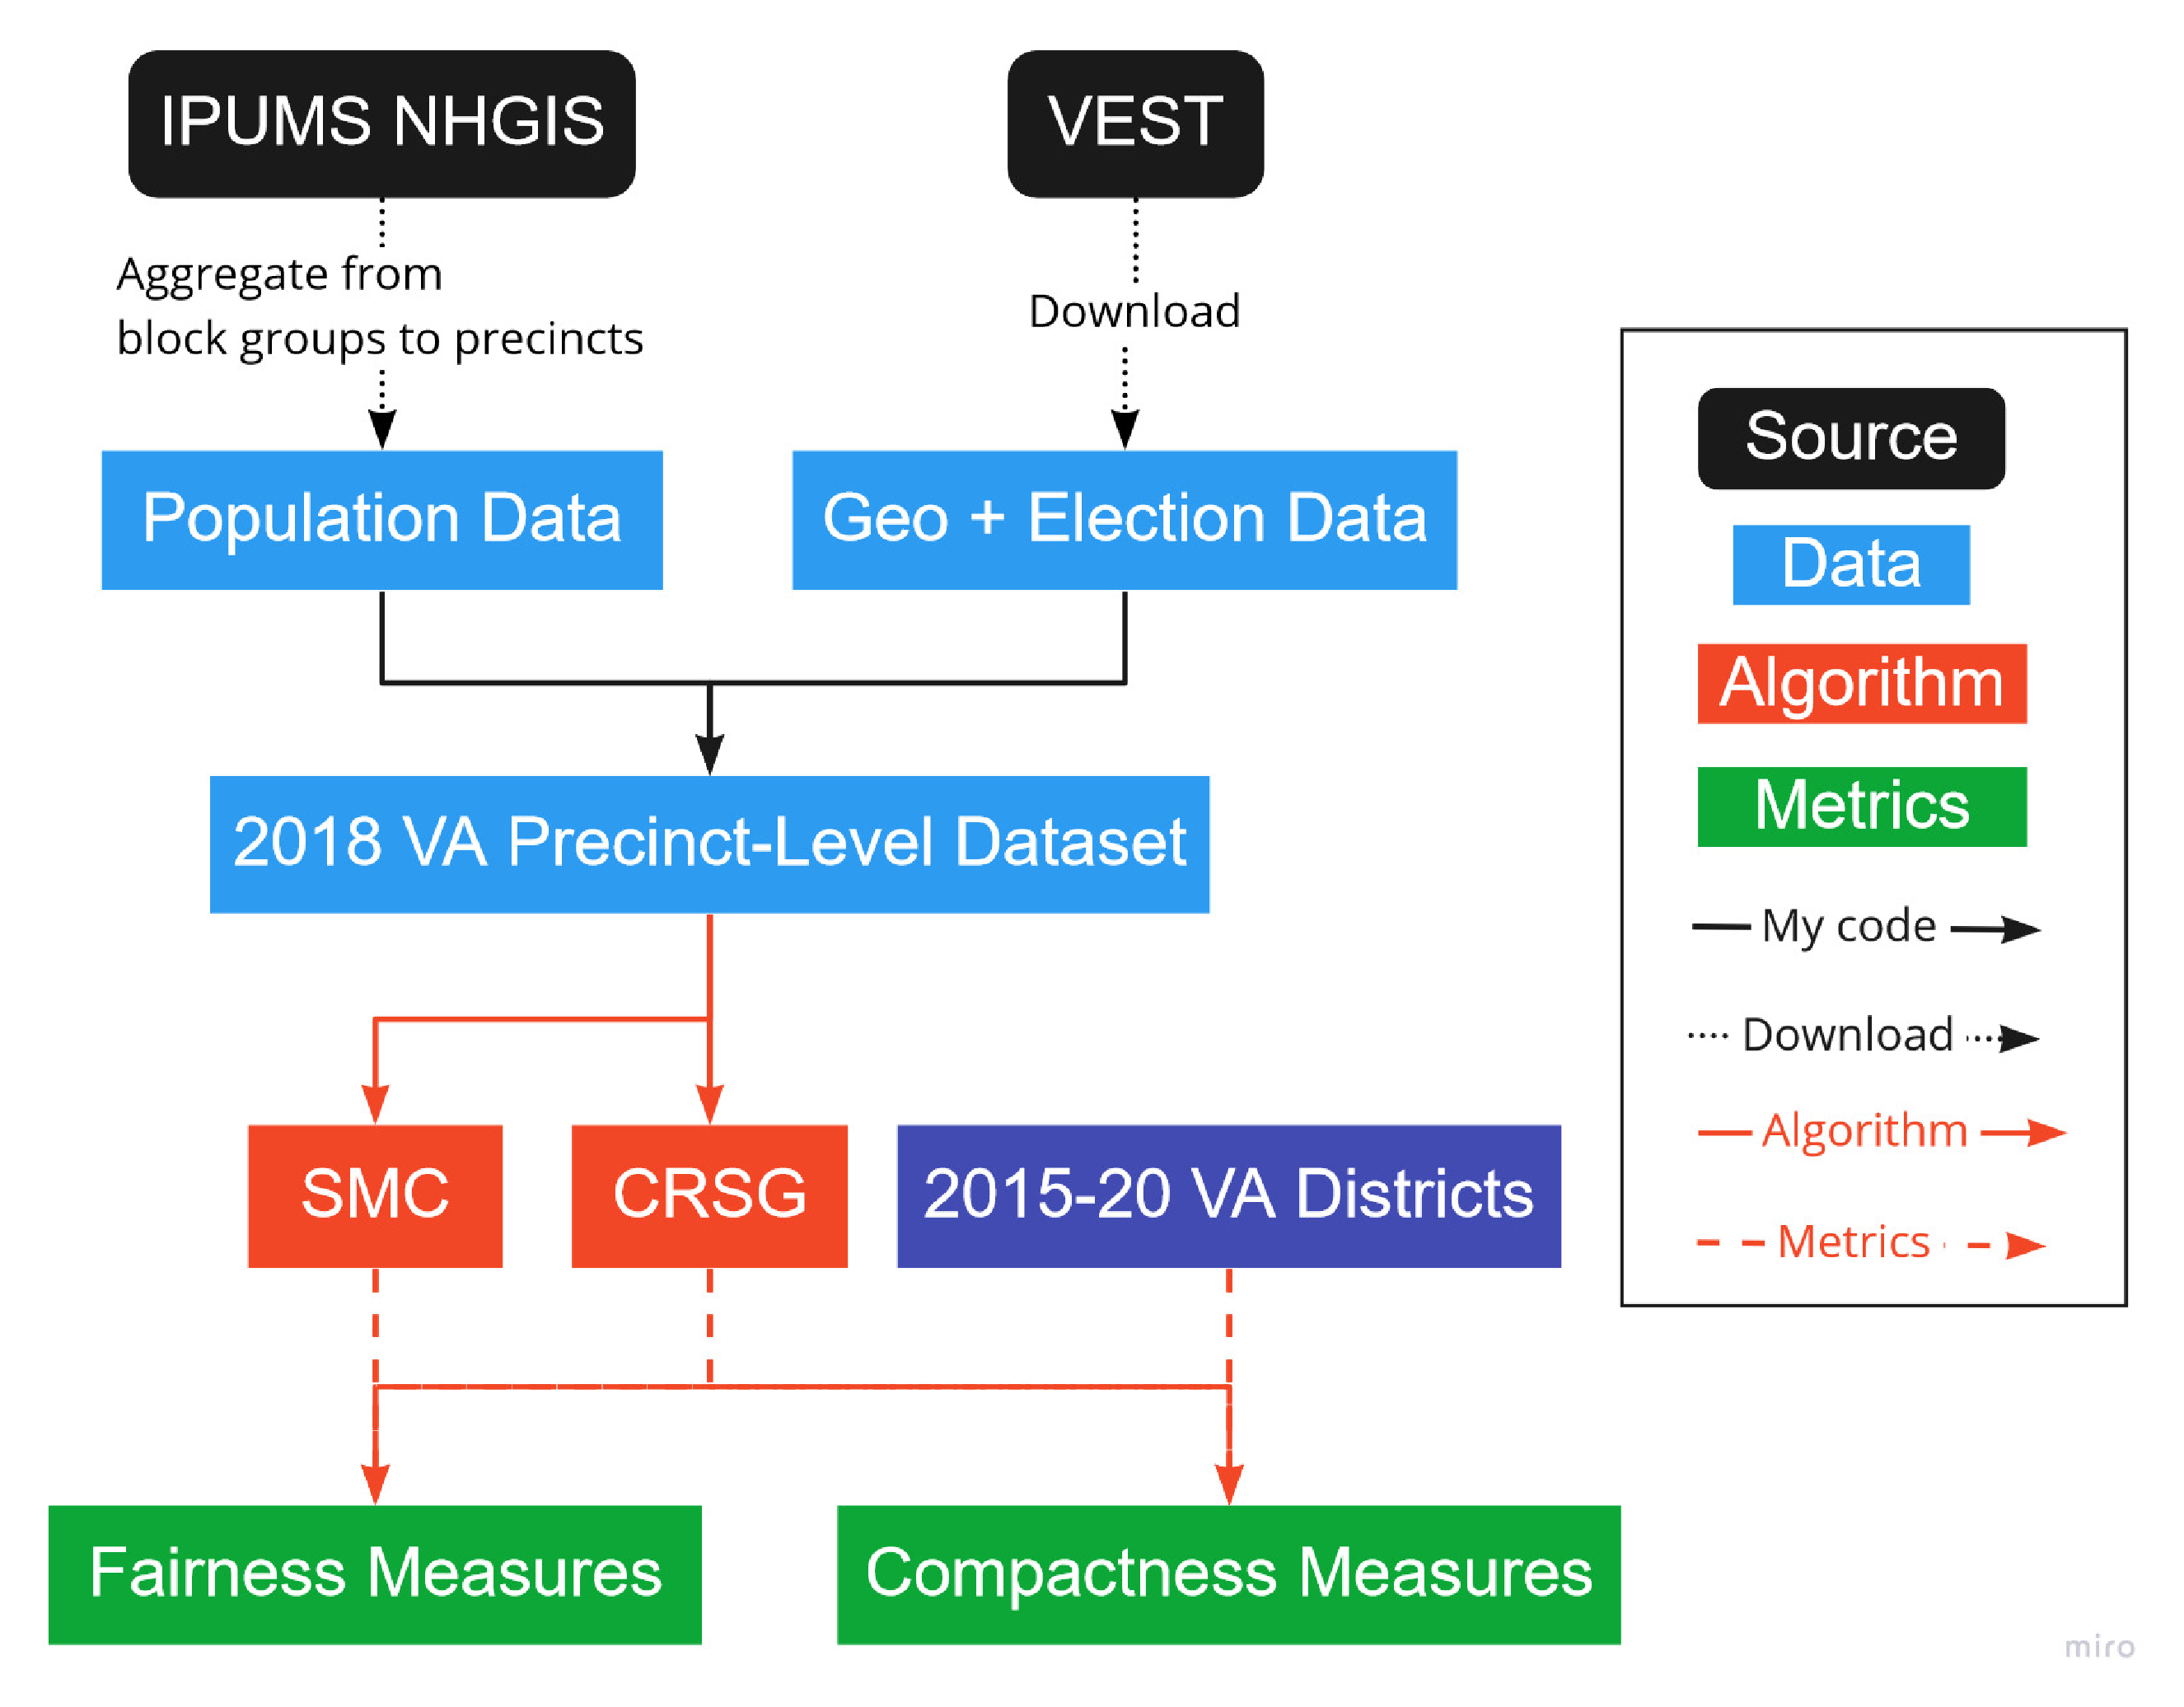
\includegraphics[width=\linewidth]{img/flowchart.pdf}
    \caption{Graphical Overview of project}
    \label{fig:flowchart}
\end{figure}

My research method simulates redistricting the legislative districts for the Virginia House of Delegates using three different algorithms in the years 2015, 2017, and 2019. Figure \ref{fig:flowchart} provides and overview of this process. I begin by explaining my overall research method, explaining how I'm aligned to both the components and principles of experimental designs, and then explaining the data collection and cleaning process.

\subsection{Choice of Research Method}

For this study, I chose to use the experimental design method because it will allow me to isolate the hypothetical impact of the redistricting algorithm from other possible confounding variables. This method also includes the use of a control group, which allows the researcher to establish causation. 

\subsubsection{Components of Experimental Design}

\paragraph{Experimental Units}

The experimental units for this study are the complete datasets for each election year in Viriginia.\footnote{This corresponds to the blue rectangles in Figure \ref{fig:flowchart}.} I have one dataset for each of these years: 2015, 2017, 2019. Every row in each dataset corresponds to a precinct, the smallest geographical unit by which votes are tabulated in Virginia. For each precinct, I have the following attributes: total population, population by race, total voting-age population (VAP)(population over the age of 18), VAP by race, total votes for the democratic House of Delegates (HOD) candidate, total votes for the Republican HOD candidate, and the total votes for any other HOD candidate. Additionally, each precinct has a polygon associated with it that represents its geographical shape. 

\paragraph{Treatments}

The treatments for this study are the three different redistricting algorithm that I'm comparing: Markov chain Monte Carlo \parencite{fifield2020}, Sequential Monte Carlo \parencite{mccartan2020}, and Random Seed Growth \parencite{chen2013}.\footnote{This corresponds to the red rectangles in Figure \ref{fig:flowchart}} I'm using the implementations in the R programming language "redist" package \parencite{fifield2020d}. See the Literature Review section for a deeper dive into these algorithms. Broadly, I chose them because they are deterministic. Much of the literature focuses on creating many possible redistricting plans for a commission to choose from, but these three aim to create an "ideal" map. 

\paragraph{Response Variables}

Broadly, the goal will be to evaluate how "fair" each redistricting plan generated by each algorithm for each year is.\footnote{This corresponds to the green rectangles in Figure \ref{fig:flowchart}.} Within the literature, partisan symmetry is the primary principle used to evaluate redistricting plans. \textcite{katz2020} brings mathematical rigor to the various proposed metrics for measuring partisan symmetry. 

\subparagraph{Partisan Symmetry}

A legislative is said to have partisan symmetry if both parties can receive $m$ proportion of the overall votes and therefore have $n$ proportion of the seats in the legislative body.An example would be that if Republicans win 60\% of the votes but control 65\% of the seats, then in a symmetrical system, Democrats should also be able to control 65\% of the seats by winning 60\% of the votes. \textcite{katz2020}

\begin{figure}
    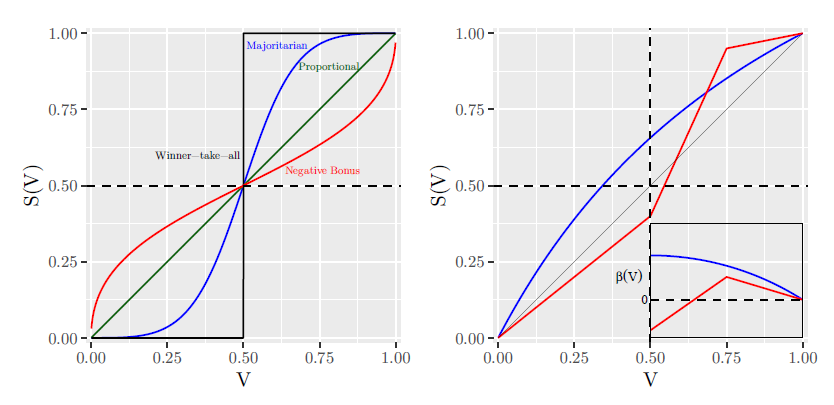
\includegraphics[width=\linewidth]{img/seatsvotes.png}
    \caption{Types of Seats-Votes Curves. Left panel: Symmetric (fair) curves with differing
    levels of electoral responsiveness. Right panel: Asymmetric (biased) curves, including
    one consistently biased toward the Democrats (blue) and one with biases favoring different
    parties depending on V (red); the inset graph is for (V ) for V 2 [0:5; 1] with the vertical
    axis scaled to be the same as the main plot, and lines color coded to the seats-votes curves. \parencite[175]{katz2020}}
    \label{fig:seatsvotes1}
\end{figure}

Partisan symmetry is usually observed by plotting a "seats-votes curve." This plot has $V$, the proportion of the overall votes won by the party, on the x-axis, and $S(V)$, the proportion of the seats won by the party, on the y-axis. Figure \ref{fig:seatsvotes1} \parencite[175]{katz2020} illustrates several hypothetical seats-votes curves.

Naturally, it's very rare to observe the necessary electoral outcomes under the same electoral system in order to determine partisan symmetry. (ie., it's very rare for two parties to tie one year, have one win 51\% of the total votes the next year, and then win 49\% of the votes the following year.)

In practice, one can estimate a seats-votes curve using the principle of uniform partisan swing.

\subparagraph{Uniform Partisan Swing}

Uniform partisan swing is the principle that when the overall vote share $V$ changes by some amount $dV$ between different elections under the same electoral system, the vote share at the district level also usually changes by the same $dV$. \textcite{katz2020} Empirically verified this to be true in 646 different elections. 

Thus, given a list of vote proportions per district ${v_1, v_2, v_3, ...}$ from one election, one can adjust each vote proportion by an arbitrarily small $dV$ until the seats share $S(V)$ is covered from 0 to 1. \parencite{katz2020}.

\begin{figure}
    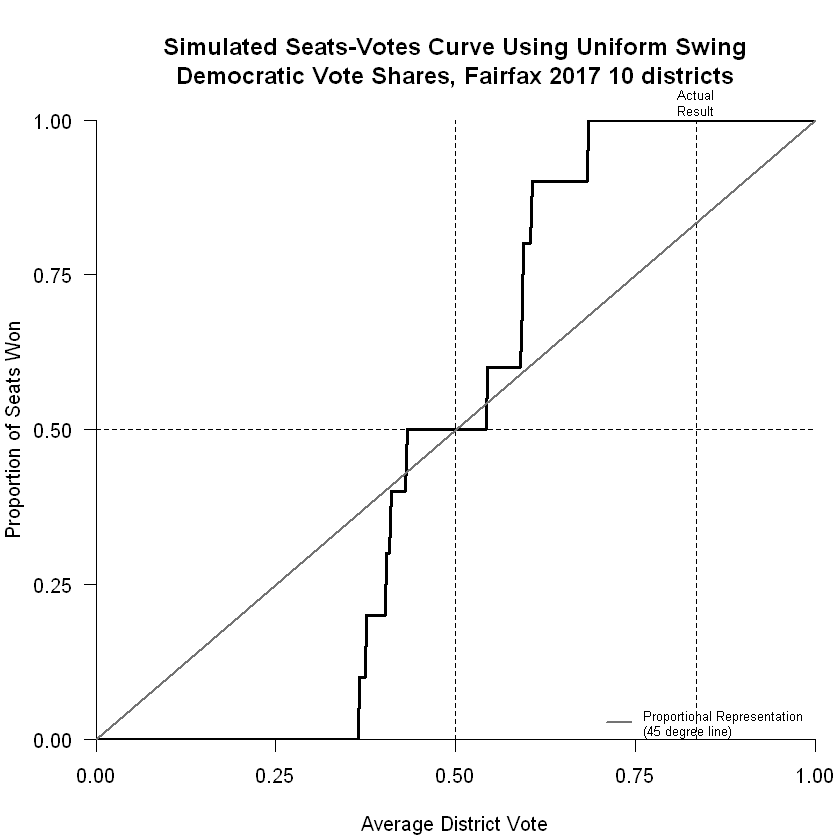
\includegraphics[width=0.5\linewidth]{img/seatsvotesups.png}
    \caption{Sample seats-votes curve generated using uniform partisan swing. Ignore title. \parencite[175]{katz2020}}
    \label{fig:seatsvotesups1}
\end{figure}

An example of such a curve is shown in Figure \ref{fig:seatsvotesups1}

\subparagraph{Chamber Power Balance}

Since the redistricting that's occuring is hypothetical and I have precinct-level election results for each of these years, I can simulate what the power distribution in the VA House of Delegates would be if the proposed redistricting plan had been used. 

\paragraph{Control Group}

The official VA House of Delegates map used in the years 2015-2019 will serve as the control group for this experiment. I will compute the same metrics for this map as I will for my hypothetical redistricting plans.\footnote{This corresponds to the purple rectangle in Figure \ref{fig:flowchart}.}

\subsubsection{Principles of Experimental Design}

The primary principles of experimental research design are randomization, replication, and local control. This is how I plan to address them. 

\paragraph{Randomization}

Every experimental unit will receive each treatment, and every experimental unit can be replicated many times without issue, so there’s no error from a lack of randomization. Think of each treatment operating within a separate parallel universe. 

\paragraph{Replication}

There is no need for me to run my trials several times (run the same algorithm on the same data set several times) because these are deterministic algorithms, and the datasets will be immutable. 

\paragraph{Local Control}

All of the redistricting will be happening in controlled environments, so there will be no way for lurking variables to creep in and confound my results. 

\subsection{Data Cleaning}

To create my datasets, I cleaned and compiled three different types of data: demographic data, Geographic Information Systems (GIS) data, and election data.\footnote{This is an explanation of the black and blue rectangles in Figure \ref{fig:flowchart} and the transitions between them.} 

\subsubsection{Demographic Data}

One required piece of data in order to redistrict is demographic data at the precinct level. This means both the total population and the Voting-Age Population (VAP) broken down into the Non-Hispanic White, Non-Hispanic Black, and Hispanic categories. In order to run the most accurate redistricting simulations, these data needed to be recent for the year being redistricted, meaning I needed different data sets for 2015, 2017, and 2019. Comprehensive population counts are only conducted by the US Census Bureau every 10 years, so I instead used the 5-year American Community Survey results at the block-group level. This is a sample survey, not a population count, but that is offset by the aggregation of sample data over a 5 year period. I downloaded this data from the IPUMS National Historic GIS project \parencite{mansonsteven2020}. Using the "maup" Python Library \parencite{hully}, I disaggregated the data from the block-group level to the block level, prorating the demographic data based on population. This data was then aggregated up to the precinct level.

However, IPUMS did not have VAP by race data, so I downloaded that separately from the US Census Bureau \parencite{uscensusbureau} and cleaned it in a similar fashion, merging it into my precinct tables. 

\subsubsection{GIS Data}

In order to redistrict, the algorithms need to know the shape and relative location of each precinct. In practice, this means every precinct has a "polygon" associated with it and a Coordinate Reference System that describes where these polygons fall in space. These data tables with the geometry column are known as "shapefiles." I accessed these shapefiles from the Voting and Election Science Team on their Harvard Dataverse \parencite{votingandelectionscienceteam2019a,votingandelectionscienceteam2019,votingandelectionscienceteam2019b}. I then merged in my precinct-level demographic data tables, so I now have shapefiles with the necessary demographic data. \footnote{Since election administrators are free to change the precincts between elections, precinct shapefiles are unique to both a place and a time. This was the reason that I only ran simulations in the years 2015, 2017, and 2019, since these were the only years for which I was able to find reputable precinct shapefiles.}

\subsubsection{Election Data}

The last necessary component needed to evaluate redistricting plans is the number of votes one by each party in each precinct in each election.\footnote{The algorithms I'm comparing assume a 2 party system, so I only tracked Democratic and Republicn votes won in each election.} The Virginia Department of Elections publishes historical records of every election on their website \parencite{virginiadepartmentofelections}, which I cleaned and aggregated to arrive at a party vote count for each precinct for each year. These data were then merged into my precinct shapefiles.